\documentclass{beamer}
\usepackage[utf8]{inputenc}
\usepackage{babel}
\usepackage{amsmath}
\usepackage{tikz}
\usetikzlibrary{positioning,chains,fit,shapes,calc}
\usepackage{minted}

\usepackage{hyperref}
\hypersetup{
    colorlinks=true,
    linkcolor=blue,
    filecolor=magenta,      
    urlcolor=cyan,
}
\urlstyle{same}

\setlength{\parskip}{1em}

\title{What Is \LaTeX?}
\author{Jesse He}
\institute{OSU MMC Project Group}
\date{2020}

\begin{document}

\frame{\titlepage}

\begin{frame}{What is \LaTeX?}
    \pause \LaTeX{} is a document preparation tool commonly used in
    \href{https://arxiv.org/pdf/2001.00683.pdf}{mathematics},
    \href{https://arxiv.org/pdf/2001.00863.pdf}{physics},
    \href{https://arxiv.org/pdf/1912.13122.pdf}{computer science},
    \href{https://arxiv.org/pdf/2001.00921.pdf}{statistics},
    and \href{https://arxiv.org/pdf/1912.13167.pdf}{many}
    \href{https://arxiv.org/pdf/1912.12611.pdf}{other}
    \href{https://arxiv.org/pdf/2001.00889.pdf}{fields}
    to typeset academic papers, lecture notes, and presentations (like this one!)
    
    \pause
    The purpose of this project group will be to introduce you to \LaTeX{} and
    to give you some familiarity with using it to prepare a document.
\end{frame}

\begin{frame}{What can you do in \LaTeX?}
    \pause
    Well...
    
    \pause
    \LaTeX{} is \href{https://en.wikipedia.org/wiki/Turing_completeness}{Turing complete},
    so technically you can do just about anything in it!

    \pause
    A better question might be:
    \pause
    What \textit{should} you do in \LaTeX?
\end{frame}

\begin{frame}{What is \LaTeX{} good for?}
    \pause
    \LaTeX{} is a document preparation tool, so you can use it anywhere you would normally use
    Microsoft Word or Google Docs.
    
    \pause
    \LaTeX{} is especially handy if you need to typeset math that looks like this:
    \[
        \oint_{\partial R} \mathbf{F} \,d\mathbf{x} = \int \int_R \nabla \times \mathbf{F} \cdot \,dR
    \]
    
    \pause
    or you want a diagram that looks like this:
    \begin{center}
    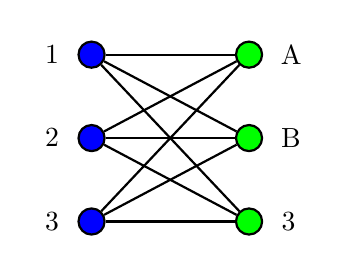
\begin{tikzpicture}[thick,
      every node/.style={draw,circle},
      fsnode/.style={fill=blue},
      ssnode/.style={fill=green}
    ]
    
    % the vertices of U
    \begin{scope}[start chain=going below,node distance=7mm]
    \foreach \i in {1,2,3}
      \node[fsnode,on chain] (f\i) [label=left: \i] {};
    \end{scope}
    
    % the vertices of V
    \begin{scope}[xshift=2cm,start chain=going below,node distance=7mm]
    \foreach \i in {A, B, 3}
      \node[ssnode,on chain] (s\i) [label=right: \i] {};
    \end{scope}
    
    % the edges
    \foreach \i in {1, 2, 3}
        \foreach \j in {A, B, 3}
            \draw (f\i) -- (s\j);
    \end{tikzpicture}
    \end{center}
\end{frame}

\begin{frame}[fragile]{What is \LaTeX{} good for?}
    \LaTeX{} also supports code highlighting:
    \begin{minted}[fontsize=\footnotesize]{python}
# Insertion sort implemented in python
def insertion_sort(data) :
	for i in range(1, len(data)) :
		j = i
		while j > 0 and data[j-1] > data[j] :
			data[j], data[j-1] = data[j-1], data[j]
			j -= 1
	return data
    \end{minted}
\end{frame}

\begin{frame}[fragile]{Why use \LaTeX?}
    \pause
    Unlike Word or Docs, which are What-You-See-Is-What-You-Get (WYSIWYG) editors,
    \LaTeX{} is a \textbf{markup} language.
    
    \pause
    That means that in \LaTeX, a mathematical formula like the one we saw earlier that looks like this
    \[
        \oint_{\partial R} \mathbf{F} \,d\mathbf{x}
        = \int \int_R \nabla \times \mathbf{F} \cdot \,dR
    \]
    is generated by typing this:
    \pause
    \begin{minted}{latex}
\[
    \oint_{\partial R} \mathbf{F} \,d\mathbf{x}
    = \int\int_R \nabla\times\mathbf{F} \cdot \,dR
\]
    \end{minted}
\end{frame}

\begin{frame}{Why use \LaTeX?}
    This means that \LaTeX{} can be a little harder to learn, but it becomes really useful for
    typesetting documents with lots of formulas or diagrams that are hard to format in a WYSIWYG
    editor.
    
    \pause
    \LaTeX's capabilities can also be extended with \textbf{packages}, which we will discuss later.
\end{frame}

\begin{frame}{How do you get started with \LaTeX?}
    \pause
    There are two main ways to use \LaTeX:
    \begin{enumerate}
        \pause \item You can use a free online service like Overleaf
        \pause \item You can install a local distribution onto your computer
    \end{enumerate}
    \pause
    For our purposes, we will use Overleaf since it's easier to start with.
\end{frame}

\begin{frame}{For next week}
    \begin{enumerate}
        \item Make sure you have created an Overleaf account
        \item Explore! You can find documentation for basic tasks at
            \url{https://www.overleaf.com/learn}, or you can simply experiment with a blank document
    \end{enumerate}
\end{frame}

\end{document}
